\documentclass{article}
\usepackage[utf8]{inputenc}
\usepackage{graphicx}
\usepackage{amsmath}
\usepackage{geometry}

\geometry{margin=0.5in}

\newcommand{\bra}[1]{\langle#1|}
\newcommand{\ket}[1]{|#1\rangle}

\title{Helical Ladder Model}
\author{Jack Crewse}
\date{September 2022}

\begin{document}

\maketitle

\section{Introduction}
The goal in this set of notes is to understand the simulation of a `helical ladder' system - consisting of a two atom unit cell which features screw dislocations along an axis which extends to infinity (e.g. similar to the DNA double helix) - using the \verb|kwant| quantum transport simulation package. This simulation is intended to be the starting point for understanding the simulation of general helical materials consisting of 'bulk' 2D materials stacked with a twist angle between layers. 

\section{Simple Ladder Model}
To get started, we first simulate a simple ladder system (two atom units cell without the screw dislocation). This has a relatively simple Hamiltonian (in atomic units $\hbar = m = c = 1$) in the tight-binding approximation
\begin{align}
    H_{SL} & = u\sum_{i,j} \ket{i,j}\bra{i,j} \label{eqn:simple-on-site} \\
       &- t\sum_{i,j} \big[\ket{i,j}\bra{i,j+1} + \ket{i,j+1}\bra{i,j}\big] \label{eqn:simple-intralayer-hop} \\
       &- v\sum_{i,j} \big[\ket{i,j}\bra{i+1,j} + \ket{i+1,j}\bra{i,j}\big] \label{eqn:simple-interlayer-hop} \\
       &- w\sum_{i} \big[\ket{i,0}\bra{i+1,1} + \ket{i+1,1}\bra{i,0} + \ket{i,0}\bra{i-1,1} + \ket{i-1,1}\bra{i,0}\big] \label{eqn:simple-cross-hop}.
\end{align}
The first term (\ref{eqn:simple-on-site}) accounts for on-site energies $u$, the second term (\ref{eqn:simple-intralayer-hop}) accounts for hopping along the y-axis (within the layer) with hopping integral $t$, the third term (\ref{eqn:simple-interlayer-hop}) accounts for hopping along the x-axis (between layers) with hopping integral $v$, and the fourth term (\ref{eqn:simple-cross-hop}) accounts for `cross' hopping (i.e. next-nearest neighbors) with hopping integral $w$. A schematic of this system is shown in Figure \ref{fig:simple-ladder} (left) along with the system as output by \verb|kwant| (right).

\begin{figure}[ht]
    \centering
    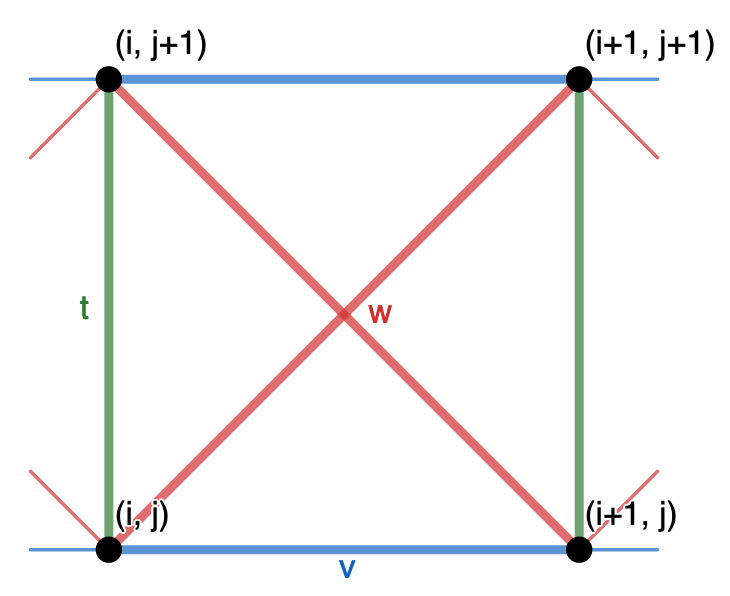
\includegraphics[width = 0.25\linewidth]{../figures/hoppings-schematic.png}
    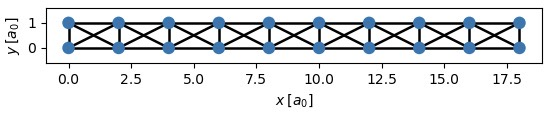
\includegraphics[width = 0.5\linewidth]{../figures/ladder_structure}
    \caption{Left: A schematic of a few sites of the ladder system defining hopping and site-labeling conventions. Right: A finite length example of the simple ladder system as output from kwant. Lengths in units of the Bohr radius.}
    \label{fig:simple-ladder}
\end{figure}

\subsection{Spectrum and wavefunctions: Finite-system}
First we consider the spectrum $\epsilon_n$ and wavefunctions $\Psi_n(x,y)$ of a few of the lowest states for the simplest case of a finite-length ladder model. Figure \ref{fig:simple-spec-wave} shows the eigenvalue spectrum and wave functions of the lowest calculated eigenenergies. The lowest state is a nodeless state and the increase in energy corresponds to an increase in the number of nodes in the wavefunctions (or probability density $|\Psi|^2$).

\begin{figure}
    \centering
    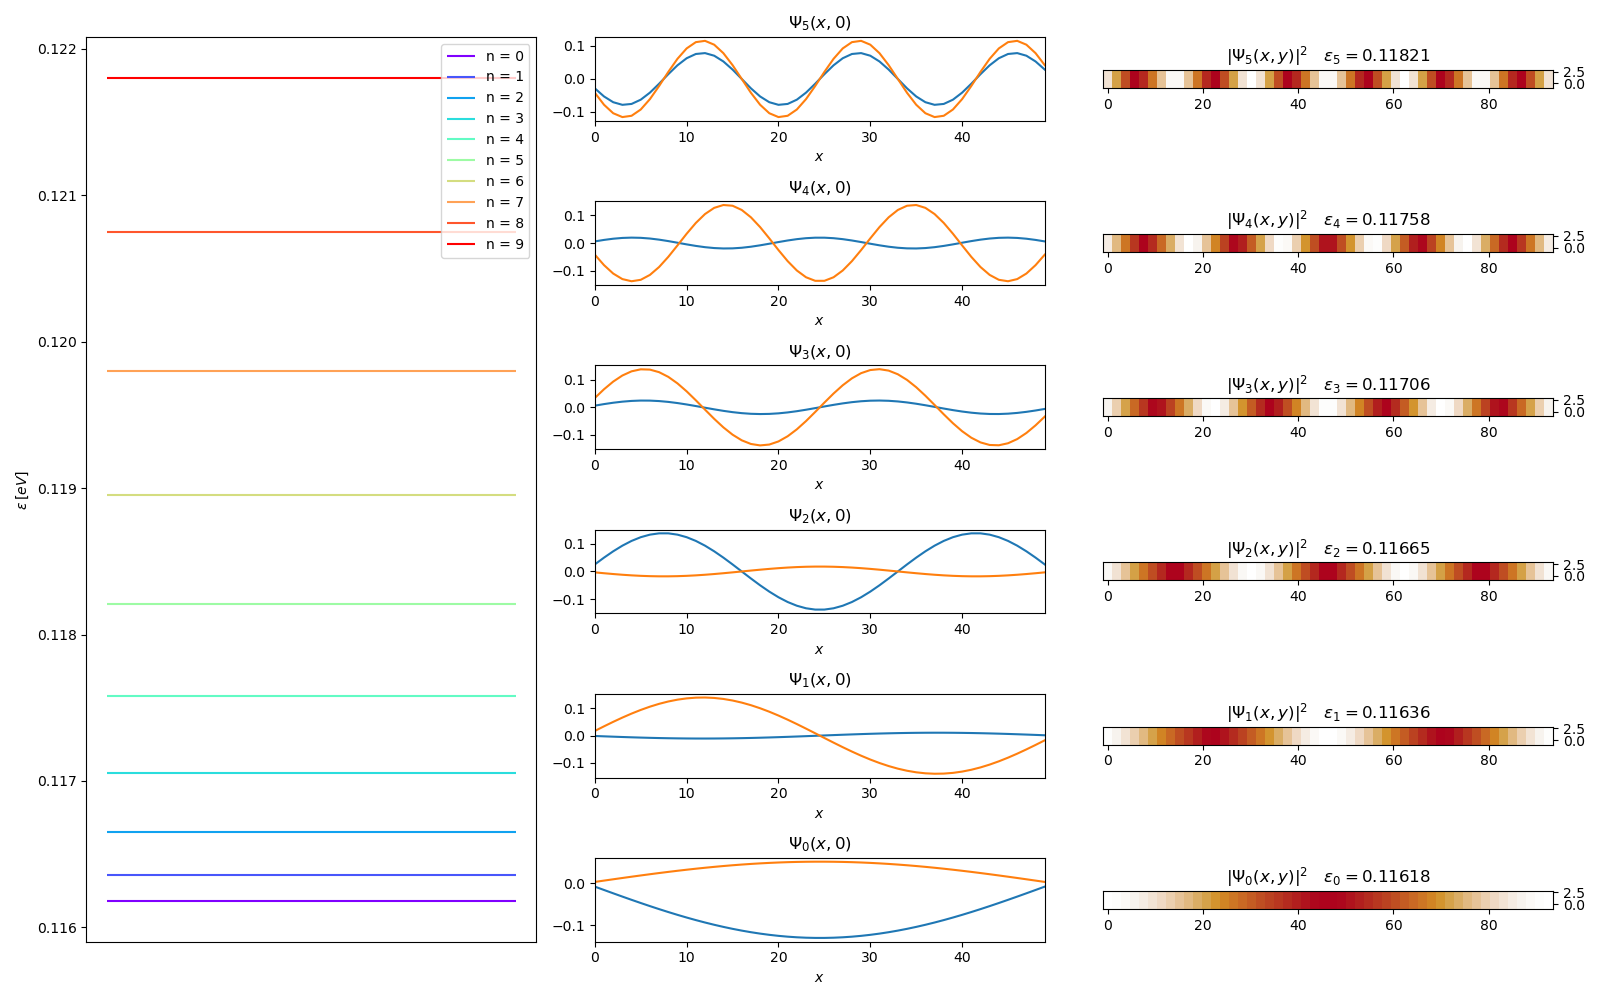
\includegraphics[width = \linewidth]{../figures/spec-wave_a1b1p0_u5t1v1w1.png}
    \caption{Left: Eigenvalue spectrum for the simple ladder model. Right: Probability density for the five lowest eigenenergies. Calculated from a system with lattice constants $a=b=1$, on-site energy $u=5$, and hoppings $t=v=w=1$.}
    \label{fig:simple-spec-wave}
\end{figure}

\subsection{Band Structure}
We first consider the most basic case of this simple ladder system. A system with equal lattice constants $a = b = a_0$ ($a_0 = $ the Bohr radius) and with no cross hoppings $w = 0$ (i.e. only nearest-neighbor hopping). The band structure for this case can be seen in figure 1 (left). As we increase the intralayer hopping parameter $t$, we see that the separation between the valence and conduction bands begins to widen because the energy difference between the 

\begin{figure}[h]
    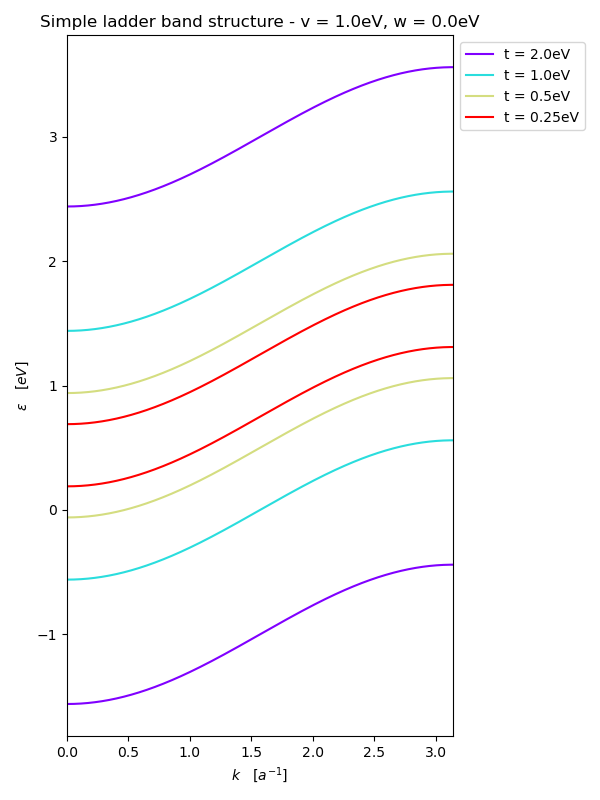
\includegraphics[width= 0.32\linewidth]{../figures/BS-vs-t_v1w0.png}
    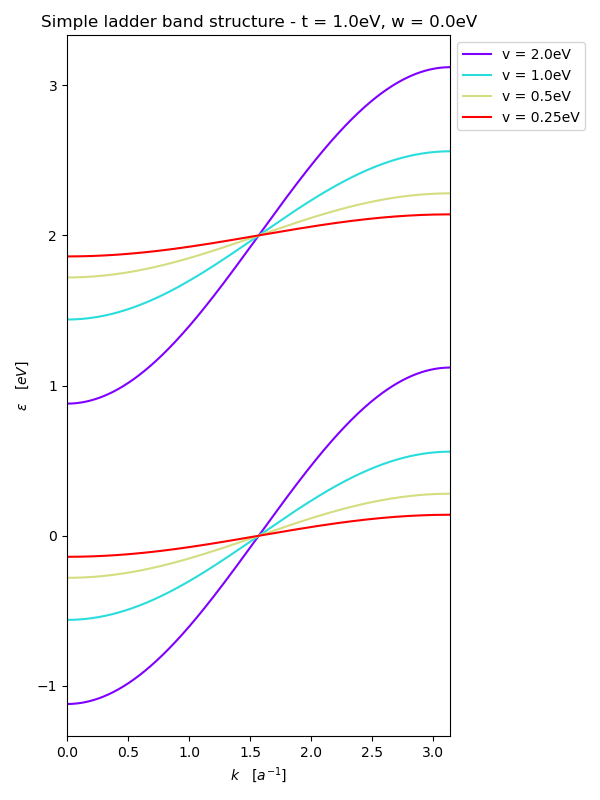
\includegraphics[width= 0.32\linewidth]{../figures/BS-vs-v_t1w0.png}
    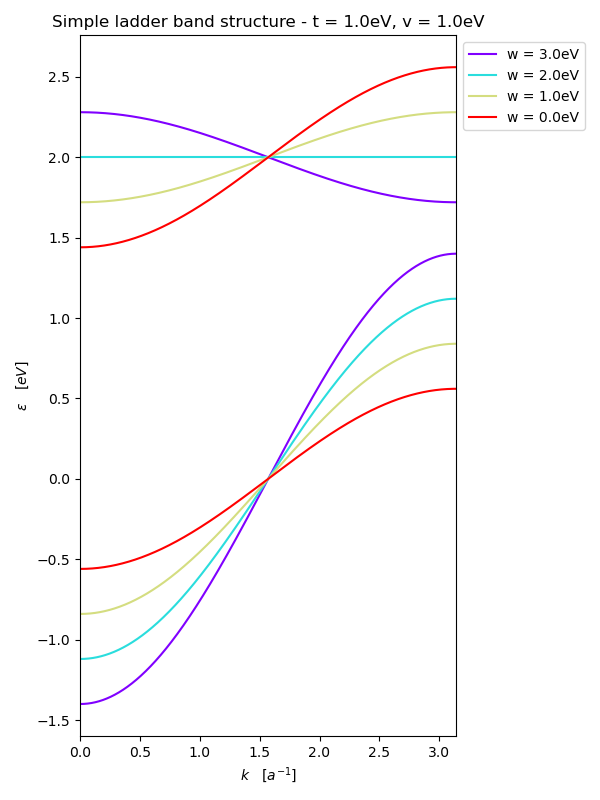
\includegraphics[width= 0.32\linewidth]{../figures/BS-vs-w_t1v1.png}
    \caption{Band structure for the simple ladder model with a fixed interlayer hopping $v = 1$ and no cross hopping $w = 0$ is on the left. As the intralayer hopping parameter $t$ is increased, the energies of both bands are increased the bandwidth and gap. The band structures for the same system but with a fixed intralayer hopping $t = 1$ and no cross hopping $w = 0$ is on the right. As the interlayer hopping parameter $v$ is varied, you can see it evolve from a highly dispersed, high-bandwidth structure $v = 5.0$ to a nearly dispersion-less, two-level system $v=0.25$ as the layers become effectively independent two atom systems.}
    \label{fig:my_label}
\end{figure}

\section{Helical Ladder Model}
Next, we want to introduce a twist angle $\phi$ into the simple ladder model along the x-axis. To implement this, instead of physically displacing the atomic locations (which is not straight-forward in \verb|kwant|), as a first approximation we simply scale the tight-binding hopping parameters $v$ and $w$ (the in-plane hopping $t$ is unaffected by the twist angle) according to the change in distance between the corresponding atoms that occurs in a rotation of $\phi$. This approximation thus maps the hopping parameters as
\begin{align}
    v(\phi) &\quad\longrightarrow\quad v/l_v(\phi) \\
    w(\phi) &\quad\longrightarrow\quad w/l_w(\phi)
\end{align}
where $l_v$ and $l_w$ represent the distances between atoms coupled via $v$ and $w$, respectively. A simple vector analysis of helical ladder with twist angle $\phi$ shows
\begin{align}
    l_v(\phi) =& \sqrt{\frac{a^2}{2}(1-\cos\phi) + b^2} \\
    l_w(\phi) =& \sqrt{\frac{a^2}{2}(1+\cos\phi) + b^2}
\end{align}

\subsection{Spectrum and wavefunctions: Finite-system}
Let's examine a finite helical ladder (i.e. with a twist angle) for a simple case of $\phi = \pi/2$. This creates a chain with each $H_2$ molecule being mutually perpendicular to the next in the chain. The results of this calculation are seen in Figure \ref{fig:helical-ladder-pi2}. Almost nothing changes about the states of the system other than seeing a slight increase in the eigenenergies. The wave functions and probability densities are almost identical. Why is this the case?

\begin{figure}[h]
    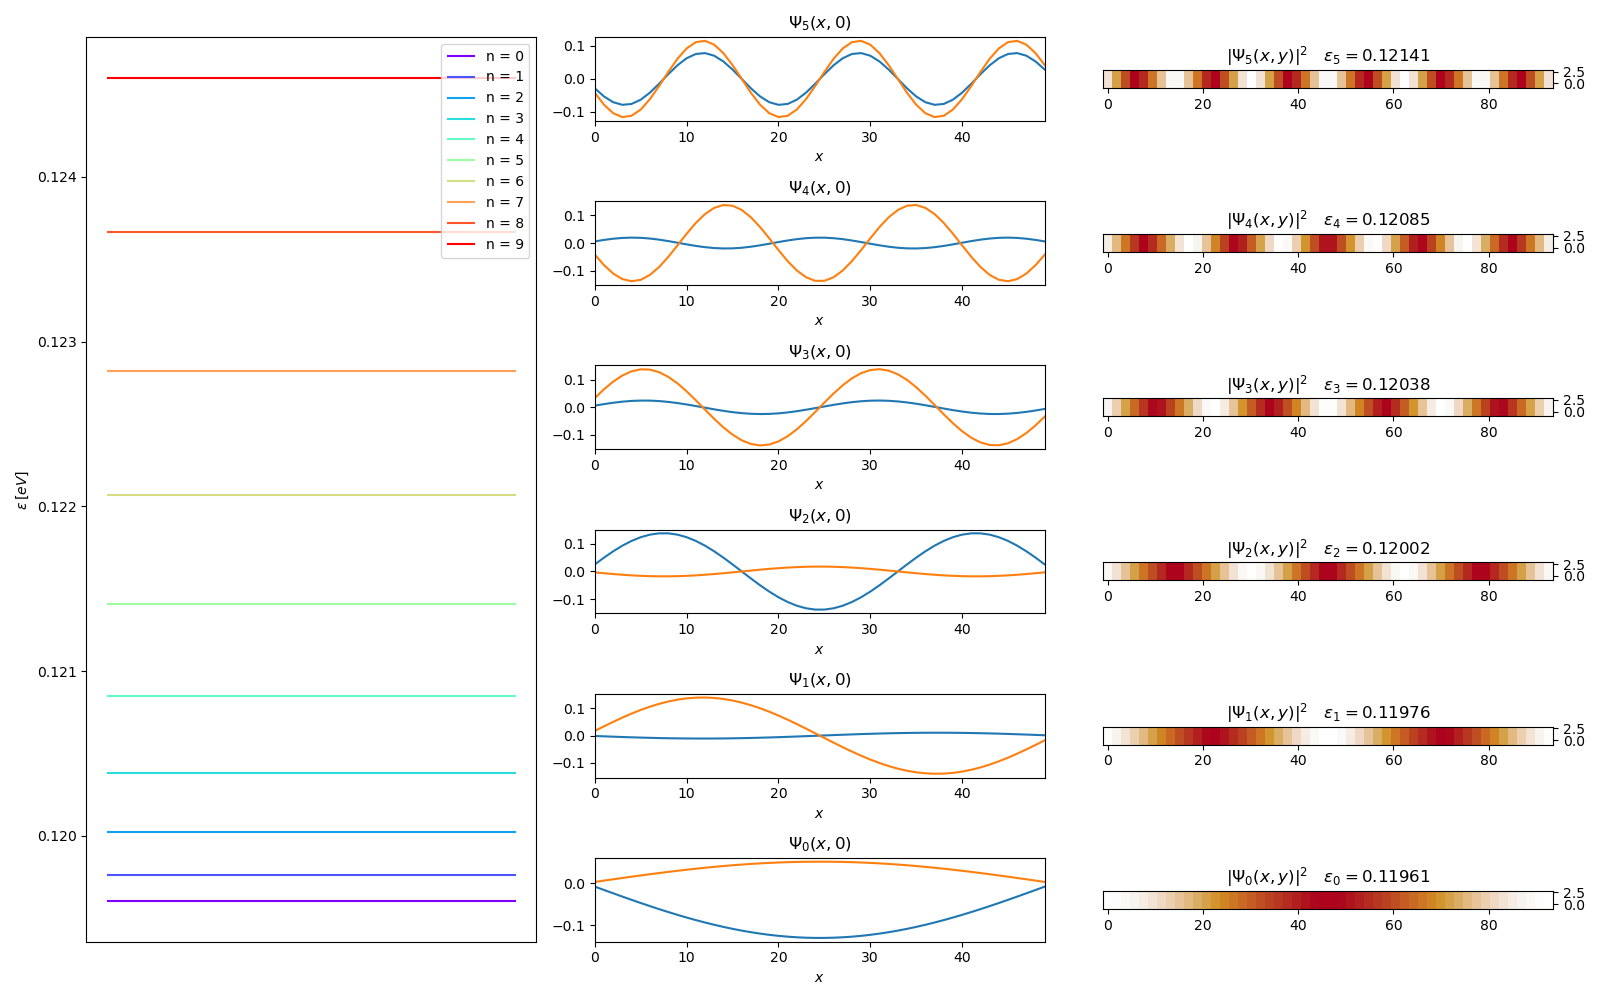
\includegraphics[width = \linewidth]{../figures/spec-wave_a1b1p2_u5t1v1w1.png}
    \caption{Helical ladder system with $\phi = \pi/2$}
    \label{fig:helical-ladder-pi2}
\end{figure}

\subsection{Band Structure}
Now let's analyze the band structure of the helical ladder for a range of twist angles. Figure \ref{fig:helical-ladder-pi2-BS} shows the results. As we can see, the upper band is heavily affected by the twist angle. It begins to invert as we increase $\phi$, becoming flat at $\phi = \pi/2, 3\pi/2$ (corresponding to a chain of  mutually perpendicular $H_2$ molecules) and completely inverting at $\phi = \pi$ (corresponding to a chain of mutually parallel $H_2$ molecules. How is this different from the original system?)

\begin{figure}
    \centering
    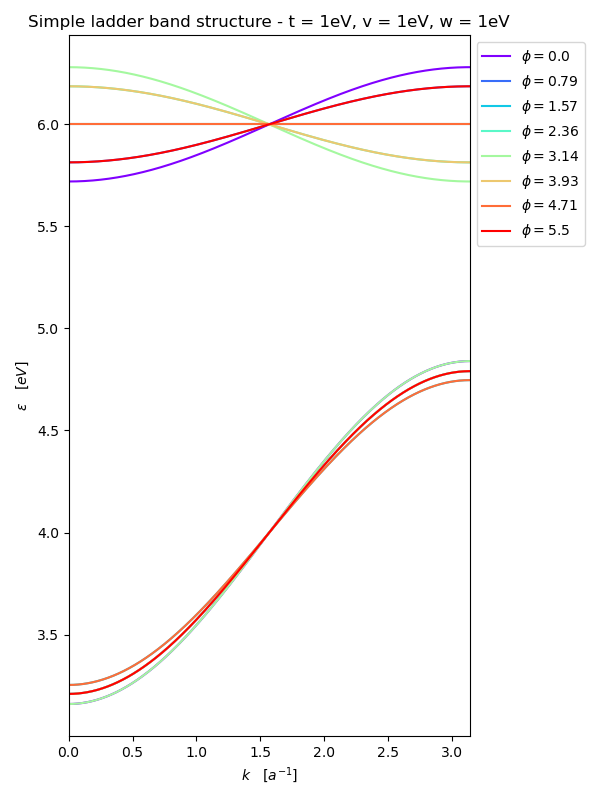
\includegraphics[scale = 0.5]{../figures/BS-vs-p_u5t1v1w1.png}
    \caption{Band structure for a helical ladder for a range of twist angles.}
    \label{fig:helical-ladder-pi2-BS}
\end{figure}

\end{document}
